% ---------------------------------------------------------------------------
% Main file. Compile with:  bash build.sh   (or: latexmk -pdf main.tex)
% The text of each section lives in sections/*.tex and was converted from
% research_paper_draft1.docx without any change to the wording.
% ---------------------------------------------------------------------------
\documentclass[10pt]{article}
% Layout and style only. No article text lives in this file.
\usepackage[T1]{fontenc}
\usepackage[utf8]{inputenc}
\usepackage{mathptmx}                 % Times-like text font
\usepackage[scaled=0.9]{helvet}
\usepackage[letterpaper,top=1in,bottom=1in,left=1.25in,right=1.25in]{geometry}
\usepackage{microtype}
\usepackage{graphicx}
\usepackage{booktabs,tabularx,array}
\usepackage[font=small,labelformat=empty,justification=raggedright,singlelinecheck=false,skip=6pt]{caption}
\usepackage{enumitem}
\usepackage{titlesec}
\usepackage{fancyhdr}
\usepackage{setspace}
\usepackage{lineno}
\usepackage{xurl}
\usepackage[hidelinks]{hyperref}
\urlstyle{same}

\newif\ifanonymous
\newif\ifsubmission

% ---- No running header; page number centered in the footer -------------------
\pagestyle{fancy}
\fancyhf{}
\fancyfoot[C]{\small \thepage}
\renewcommand{\headrulewidth}{0pt}

% ---- Headings: bold ----------------------------------------------------------
\titleformat{\section}{\normalfont\large\bfseries}{\thesection}{0.8em}{}
\titleformat{\subsection}{\normalfont\normalsize\bfseries}{\thesubsection}{0.8em}{}
\titlespacing*{\section}{0pt}{1.4em}{0.5em}
\titlespacing*{\subsection}{0pt}{1.1em}{0.3em}

% ---- Paragraphs: block style with space between paragraphs -------------------
\setlength{\parindent}{0pt}
\setlength{\parskip}{0.55em}
\setlist[itemize]{leftmargin=1.6em,itemsep=0.3em,topsep=0.3em}

% ---- Title block: centered title between two rules ---------------------------
\newcommand{\maketitleblock}{%
  \thispagestyle{fancy}%
  \vspace*{-0.5em}%
  \noindent\rule{\textwidth}{2.5pt}\par\vspace{1.0em}%
  {\centering\LARGE\bfseries \papertitle\par}%
  \vspace{0.9em}%
  \noindent\rule{\textwidth}{0.8pt}\par
  \ifanonymous\vspace{0.6em}\else
    \vspace{1.1em}%
    {\centering\normalsize\setlength{\parskip}{0pt}%
      \textbf{\paperauthor}\par
      \paperaffiliation\par
      \if\relax\detokenize\expandafter{\paperemail}\relax\else\paperemail\par\fi
      \paperdate\par
      \if\relax\detokenize\expandafter{\papercode}\relax\else \href{https://\papercode}{\papercode}\par\fi}%
    \vspace{1.6em}%
  \fi
  \ifsubmission\doublespacing\linenumbers\fi
}

% ---- Abstract and keywords ----------------------------------------------------
\newenvironment{paperabstract}{%
  {\centering\large\bfseries\scshape Abstract\par}\vspace{0.2em}%
  \begin{list}{}{\setlength{\leftmargin}{0.5in}\setlength{\rightmargin}{0.5in}}\item\relax}{\end{list}}
\newcommand{\paperkeywordsline}{%
  \begin{list}{}{\setlength{\leftmargin}{0.5in}\setlength{\rightmargin}{0.5in}}\item\relax
  \textbf{Keywords:} \paperkeywords\end{list}\vspace{0.4em}}

% ---- Tables -------------------------------------------------------------------
\newcommand{\tablesize}{\small\setlength{\tabcolsep}{5pt}}
\newcommand{\tablenote}[1]{\par\vspace{4pt}{\footnotesize\raggedright #1\par}}

% ---- Reference list: hanging indent --------------------------------------------
\newenvironment{reflist}{%
  \begin{list}{}{\setlength{\leftmargin}{1.5em}\setlength{\itemindent}{-1.5em}%
  \setlength{\itemsep}{0.35em}\setlength{\parsep}{0pt}\raggedright}}{\end{list}}

% ---- Float placement: let figures and tables share pages with text ------------
\renewcommand{\topfraction}{0.9}
\renewcommand{\bottomfraction}{0.8}
\renewcommand{\textfraction}{0.08}
\renewcommand{\floatpagefraction}{0.85}
\setcounter{topnumber}{3}\setcounter{totalnumber}{4}


% ---- Settings you can change ------------------------------------------------
\anonymousfalse         % \anonymoustrue = no author block; \anonymousfalse = show author
\submissionfalse        % \submissiontrue = double spacing + line numbers for review
\newcommand{\paperauthor}{Shannon Gross}
\newcommand{\paperaffiliation}{Independent Researcher}
\newcommand{\paperemail}{}        % optional; leave empty to hide
\newcommand{\paperdate}{Working paper, October 2026}
\newcommand{\papercode}{github.com/shannongross/ai-workforce-exposure}   % leave empty to hide
% Target journal noted in the draft (not printed):
%   nonprofit Policy Forum (NPF), published by De Gruyter Brill,
% -----------------------------------------------------------------------------

\newcommand{\papertitle}{Can AI Give Time Back? Task Exposure and Working Time\\ in Local Community Service Occupations}
\newcommand{\paperkeywords}{artificial intelligence; AI exposure; nonprofit workforce; large language models; human services; social workers}

\begin{document}
\maketitleblock

\begin{paperabstract}
Many local community service nonprofits report difficulty employing enough staff to meet rising demand for services, with rising burnout rates among workers. For those employed in this sector in food pantries, homeless shelters, child social work, the question is if the rising trend in artificial intelligence (AI) could potentially offload some of the worker burden. I examine this question for the three largest occupations in community food, housing, and relief services in the United States, combining three published task-level measures of theoretical exposure to AI, time spent per task, and observed AI use. Two of the occupations studied showed that the amount of time that large language models (LLMs) could directly speed up amounts to about a half an hour per day. A greater share of the workday (between 28-55 percent of the day) could be alleviated if additional software were built on top of the LLM for the purpose of supporting things like developing care plans and implementing training programs. These findings suggest that general-purpose AI tools are likely to return little frontline staff time, and that larger gains depend on purpose-built tools that extend LLM capability.

\end{paperabstract}
\paperkeywordsline

\section{Introduction}

Exposure to artificial intelligence (AI) in the workforce has garnered much attention in the media due to anxiety surrounding workforce displacement. However, in crucial occupational sectors that are chronically understaffed and under-resourced, there may be more optimism about AI's potential to fulfill mission objectives with less resources. Local community service organizations that provide food, shelter, and emergency relief to people in acute need persistently operate with limited staff capacity. Recent progress in large language models (LLMs), have prompted those in the sector to wonder if these tools could relieve burden for workers in this sector. For both policymakers and frontline staff, the question is how much of the working day AI might realistically support.

A growing body of literature measures how exposed work is to artificial intelligence. Eloundou et al. (2024) rate each task in the O*NET occupational database on whether an LLM could substantially reduce completion time. Hatgis-Kessell et al. (2026) add that exposure depends not only on whether AI can perform a task but on how much time workers normally spend on the task. Massenkoff and McCrory (2026) move from theoretical to observed exposure by measuring which tasks actually see work-related AI use in real Claude queries.

These studies into occupational AI exposure are broad, economy-wide analyses. For local community relief workers, this does not address the specific, practical questions around what AI exposure means for them. Research about AI in the nonprofit sector largely comes from surveys conducted about whether AI is being used (Smith Arrillaga, Grundhoefer, and Im 2025; Shi and Azevedo 2026). In cases where these surveys report how AI is used, they describe general purposes such as documentation and research (Wong et al. 2026), without linking that data to specific workforce tasks or to the time those tasks take.

In this article, I bring together existing research into theoretical AI exposure (Eloundou et al.), time per task (Hatgis-Kessell et al.), and observed AI exposure (Massenkoff and McCrory) and apply them deeply to the three largest occupations in the sector of Community Food and Housing, and Emergency and Other Relief Services (NAICS 624200). For each of these occupations, I address three questions. First, how much of the working day is directly or partially exposed to AI? Second, does measuring AI exposure by worker time versus by task count change how exposed these occupations appear? Finally, how much worker time is already showing AI use, using observed exposure data?

This analysis shows that for the three largest jobs in the local community relief services sector, there is little direct AI exposure. For instance, among Social and Human Service Assistants, the largest occupation, about 24 minutes of the entire workday could be called directly exposed to AI. Accordingly, hopes for immediate efficiency gains from AI adoption ought to be tempered. There is greater evidence for partial AI exposure, that is, if organizations were to invest in purpose-built software to enhance LLM ability, a greater share of work could likely be offloaded. The remaining half of Social and Human Service work is unexposed (unlikely to be supported by AI) due to the work being physical, interpersonal, and/or relational in nature. This article contributes a sector-focused, time-based estimate for setting realistic expectations around what AI can return in terms of staff capacity.

\section{Background}

Local community service nonprofits provide essential services, such as food pantries, homeless shelters, substance use treatment, and at-risk youth programs. More than two-thirds of nonprofits report difficulty employing enough staff (Nonprofit Finance Fund 2025). Since January 2025, 73 percent of nonprofits have seen demand for their services increase, while 30 percent have reduced staff and 29 percent have reduced services (Grundhoefer, Smith Arrillaga, and Buteau 2026). Concern about staff burnout is widespread, with ninety percent of nonprofit leaders reporting concern about burnout due to funding challenges and rising demand for services (Martin 2026). In food, shelter, and relief organizations, that strain falls largely on caseworkers and social workers, who hold more than one in five jobs (U.S. Bureau of Labor Statistics 2026). In order to improve efficiency of routine tasks, nearly two-thirds of social workers already report using AI in their work (Borah et al. 2026).

Existing research about AI in the nonprofit community service sector primarily comes from adoption surveys (Smith Arrillaga, Grundhoefer, and Im 2025; NTEN and Bridgespan 2026; Shi and Azevedo 2026). Such surveys are largely aimed at the organizational level of AI usage, and do not translate usage to the level of individual employee time. In a 2026 survey of social workers, 64\% reported using AI in their job, mostly for documentation and reporting (Borah et al. 2026). Few social workers (\textless5\%) reported using AI for more time-consuming tasks such as case management -- ethical and data privacy concerns were cited as the most common reason (Borah et al. 2026). In short, while AI has the potential to offload burden at tasks such as reporting, clerical tasks, digital work, etc. that are part of community service occupations- time-sensitivity weighting highlights that such tasks take up a relatively small part of these occupations, and so AI exposure may be lower than indicated by task-weighting alone. Much of the nonprofit worker's time involves interpersonal interaction, which takes up more of the worker's time and is less AI-exposed.

In studying theoretical ability of AI to perform workforce tasks, Eloundou et al. (2024) rate each O*NET task on whether an LLM could cut its completion time by at least half at equal quality. A task is rated directly exposed (E1) if an LLM alone could achieve that reduction, partially exposed (E2) if the LLM could do it if additional software were built on the model, and not exposed (E0) otherwise. They developed exposure scores for every O*NET task in the database, providing a foundation for analyzing theoretical exposure to AI in the workforce. A problem with using these rankings directly when studying community service nonprofits, however, is that the Eloundou et al. scores are provided per task (i.e. ``driving'', ``submit reports'', ``assist in locating housing''), they do not take into account how much time workers actually spend per task.

In "Estimating Time Spent on Work Tasks," Hatgis-Kessell et al. propose a method for weighting tasks by time for every O*NET occupation, facilitating the computation of worker time exposed to AI, rather than just the share of worker tasks exposed. Hours are the product of O*NET-reported task frequency and a per-instance duration estimated from language-model pairwise comparisons, fitted to a 7-hour working day. I apply the Hatgis-Kessell et al. approach to get to the fraction of working time (rather than the fraction of tasks) to understand AI exposure for local community relief work.

Massenkoff and McCrory (2026) move from studying theoretical to observed exposure by measuring which O*NET tasks are currently seeing work-related use, measured from conversations with Claude. Again, information is provided for the entire O*NET database at the task level. Unlike surveys which rely on humans to accurately self-report, this data is drawn from recorded use. The research from Massenkoff and McCrory indicate that actual AI use in occupations falls well short of what AI could theoretically be doing. The authors attribute this gap to factors not captured by theoretical exposure studies, namely: legal constraints, the potential need for additional software, or the time it takes to check AI results.

Existing AI exposure studies each answer a different question. Theoretical exposure work from Eloundou et al. indicate which tasks AI might speed up. Time-weighting analysis from Hatgis-Kessell et al. looks at how much time each task takes. Observed exposure from Massenkoff and McCrory indicate where LLMs are already being used compared against where they theoretically could be used. This paper adds value to the current literature by combining three different economy-scale exposure studies and applying them deeply to understand the implications for local community food, housing, and emergency service work.

\section{Methods}

\subsection{Scope and Unit of Analysis}

The population of interest in this study are organizations that provide material assistance (food, shelter, and emergency relief) to local community members. I identify these organizations using the National Taxonomy of Exempt Entities (NTEE), the classification system for US nonprofits, selecting the codes for food programs and food banks (K30 to K36), homeless and family violence shelters (L41, P43), and emergency assistance (P60). Table 1 lists the codes and their corresponding industries under the crosswalk to the North American Industry Classification System (NAICS) maintained by the National Center for Charitable Statistics.

\begin{table}[!htbp]
\tablesize
\caption*{\textbf{Table 1.} NTEE codes and corresponding NAICS industries.}
\begin{tabularx}{\textwidth}{@{}l l l X@{}}
\toprule
NTEE code & Organization type & NAICS code & NAICS industry \\
\midrule
K30 & Food Programs & 624210 & Community Food Services \\
K31 & Food Banks, Pantries & 624210 & Community Food Services \\
K34 & Congregate Meals & 624210 & Community Food Services \\
K35 & Soup Kitchens & 624210 & Community Food Services \\
K36 & Meals on Wheels & 624210 & Community Food Services \\
L41 & Homeless Shelters & 624221 & Temporary Shelters \\
P43 & Family Violence Shelters & 624221 & Temporary Shelters \\
P60 & Emergency Assistance & 624230 & Emergency and Other Relief Services \\
\bottomrule
\end{tabularx}
\end{table}

These organizations all fall in the Bureau of Labor Statistics (BLS) 4-digit industry group NAICS 624200: Community Food and Housing, and Emergency and Other Relief Services. This sector comprises 193 occupations and 231,040 jobs. For purposes of the deep dive of this study, I examine the three largest occupations by employment within this sector, which are: Social and Human Service Assistants (SOC 21-1093), Child, Family, and School Social Workers (SOC 21-1021), and Social and Community Service Managers (SOC 11-9151). Together they account for 27.6 percent of jobs within NAICS 624200. For each job, the Occupational Information Network (O*NET) provides a breakdown of the tasks that are included in each job description.

\begin{table}[!htbp]
\tablesize
\caption*{\textbf{Table 2.} Employment in the three occupations examined.}
\begin{tabularx}{\textwidth}{@{}l >{\raggedright\arraybackslash}X r >{\raggedleft\arraybackslash}p{2.7cm} >{\raggedleft\arraybackslash}p{1.3cm}@{}}
\toprule
SOC code & Occupation & Jobs & Share of NAICS 624200 jobs (\%) & O*NET tasks \\
\midrule
21-1093 & Social and Human Service Assistants & 36,250 & 15.7 & 19 \\
21-1021 & Child, Family, and School Social Workers & 13,940 & 6.0 & 21 \\
11-9151 & Social and Community Service Managers & 13,680 & 5.9 & 16 \\
& Total, three occupations & 63,870 & 27.6 & 56 \\
& Total, NAICS 624200 (193 occupations) & 231,040 & 100.0 & \\
\bottomrule
\end{tabularx}
\tablenote{\emph{Note:} SOC = Standard Occupational Classification.}
\end{table}

\subsection{Source of Data}

This study combines the following publicly available sources:

\begin{itemize}
\item
  \emph{Occupational employment.} Employment by occupation in NAICS 624200 comes from the May 2025 employment statistics from U.S. Bureau of Labor Statistics. I use these data to identify the three largest occupations in the sector.
\item
  \emph{Task descriptions.} Each occupation's tasks come from the O*NET 31.0 database, which lists 19 tasks for Social and Human Service Assistants, 21 for Child, Family, and School Social Workers, and 16 for Social and Community Service Managers.
\item
  \emph{Theoretical exposure.} Task-level exposure ratings come from Eloundou et al. (2024). A task is rated E1 if an LLM could cut the task completion time by half (directly exposed), E2 if the LLM could do it if additional software were built on the model (partially exposed), and E0 if the LLM could not do the task (not exposed). The data from this study include two ratings of every task, one by human annotators and one by GPT-4. I use the human scores as the reported measure throughout this study. I check the final results against the GPT-4 scores for robustness.
\item
  \emph{Time per task}. Estimated hours per task come from Hatgis-Kessell et al. (2026), across each occupation's O*NET tasks. I use the task-level results made publicly available by the authors.
\item
  \emph{Observed use.} Observed exposure data comes from Massenkoff and McCrory (2026), who measure work-related use of Claude per O*NET task. I use both their task-level results, published in the Anthropic Economic Index dataset via Hugging Face.
\end{itemize}

\subsection{Procedure}

I combined these data sources using SOC codes and O*NET task identifiers, so that every task in the three occupations included in this study carries an exposure rating, an estimate of daily hours, and a measure of observed use.

\begin{itemize}
\item
  Exposed time per worker. Per each of the tasks included in the three occupations of this study, I extracted the theoretical exposure metrics from Eloundou et al. (2024): directly exposed (E1), partially exposed (E2), and not exposed (E0).
\item
  Task-weighting vs time-weighting. I incorporated time-weighting as defined in Hatgis-Kessell et al. (2026) in order to compare E1, E2, and E0 against task counts per occupation.
\item
  Observed exposure. To gain more context around AI exposure, I also extracted observed AI usage per occupational task from Massenkoff and McCrory (2026).
\item
  Worker hours. For each occupation, I multiplied hours by the size of the workforce to obtain exposure in terms of worker hours per day. Note that E1 (direct exposure) and E2 (partial exposure) do not show the time that AI would save, they indicate the theoretical ability of the LLM to shorten the task by half. I do not report worker time savings due to partial exposure, since these savings depend on the creation of software that does not exist yet.
\end{itemize}

\section{Results}

The two frontline occupations (Social and Human Service Assistants and Child, Family and School Social Workers) have little of their working day exposed to AI. The managerial occupation Social and Community Service Managers shows more direct exposure to AI. In all three occupations studied, the greater share of exposure is indirect, meaning that LLMs could support the task if dedicated software were built to support it. The following sections present working time in each exposure category (4.1), compare time-weighted vs task-weighted exposure (4.2), describe observed patterns of LLM use (4.3), and present exposure results at the scale of the workforce.

\subsection{Exposed working time}

Social and Human Service Assistants spend about 24 minutes per day on tasks that could be classified as directly exposed to AI (Figure 1). That directly exposed time is spread across six small tasks, the largest being referring clients to other agencies (10 minutes per day) and submitting reports to a supervisor (9 minutes per day). A further 2 hours, 51 minutes per day fall on three tasks that are exposed only with additional software: developing care plans (1 hour, 48 minutes), locating housing (32 minutes), and keeping records of client visits (31 minutes). The remaining 3 hours 45 minutes, more than half the 7-hour workday, are not exposed. These include assessing client needs, supervising group activities, and interviewing families.

\begin{figure}[!htbp]
\centering
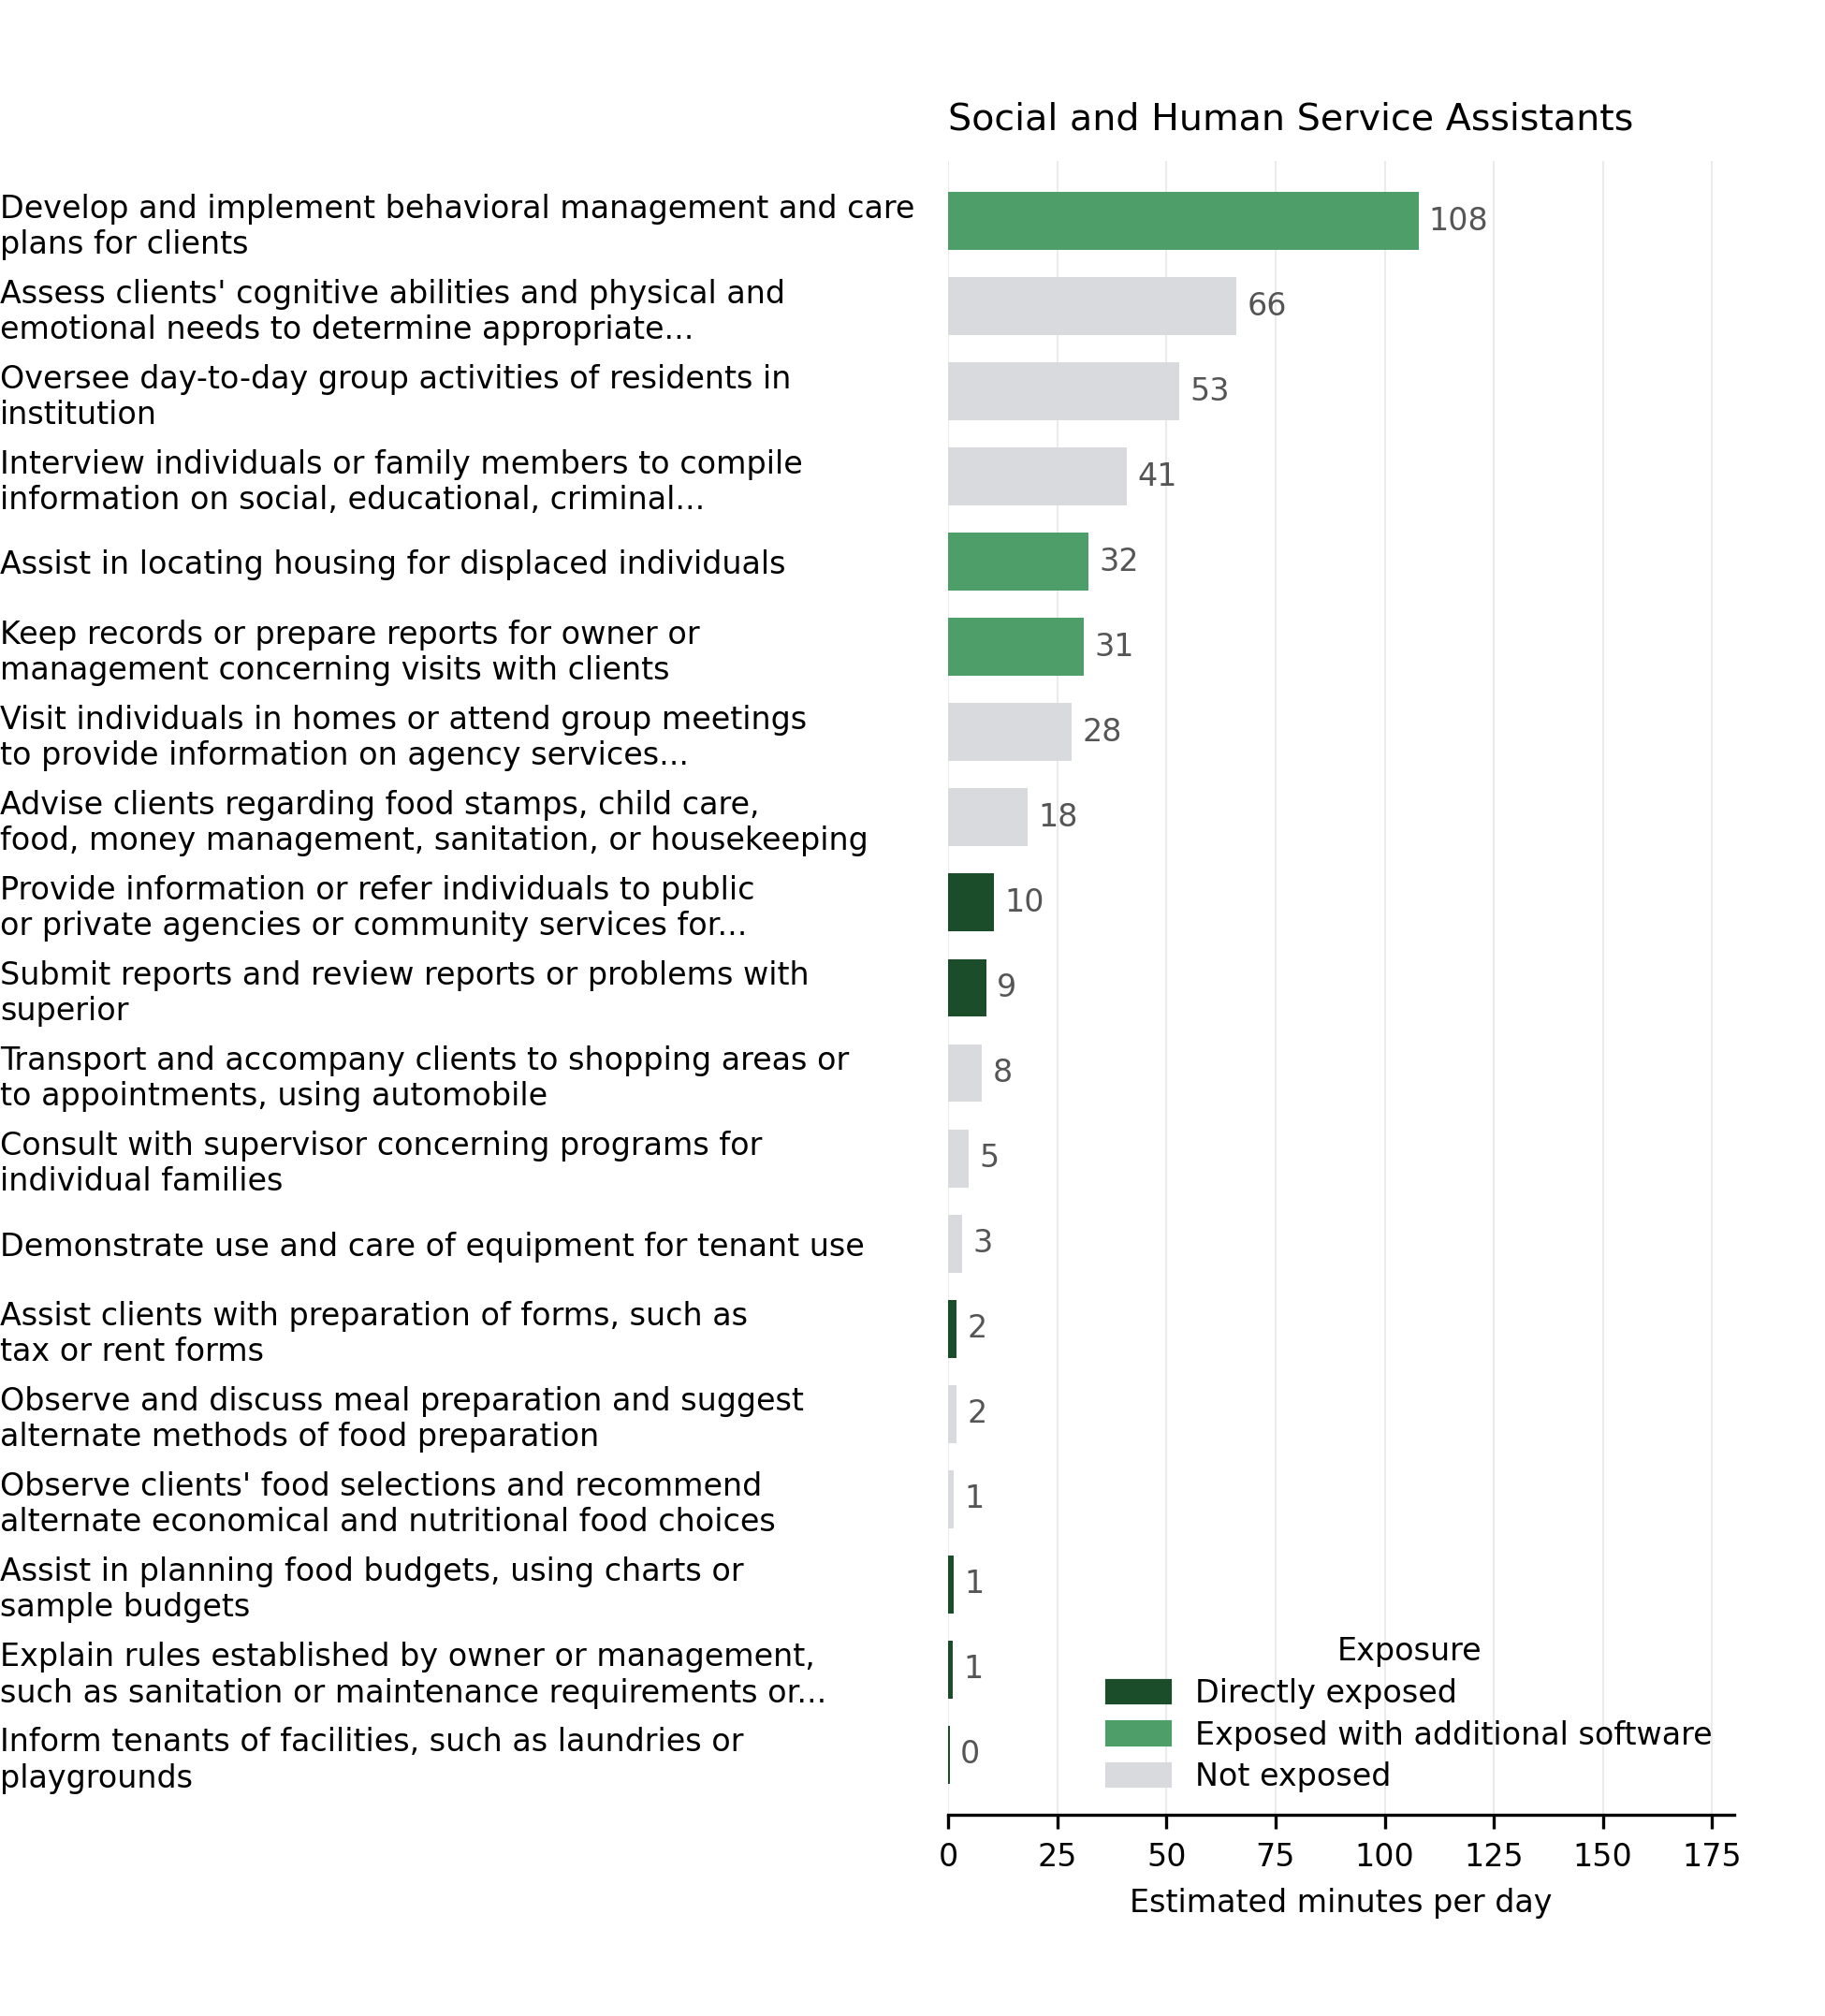
\includegraphics[width=0.8\textwidth]{figures/fig1_assistants.png}
\caption*{Figure 1: Theoretical task-based exposure to AI for Social and Human Service Assistants. Ratings are human ratings from Eloundou et al. (2024); hours from Hatgis-Kessell et al. (2026).}
\end{figure}

Child, Family, and School Social Workers show a similar pattern (Figure 2). The total amount of time a worker spends on directly exposed tasks is about 36 minutes per day. One task, "Counsel students whose behavior, school progress, or mental or physical impairment indicate a need for assistance, diagnosing students' problems and arranging for needed services" takes up 26 of those directly exposed minutes. Time on partially exposed tasks take an additional 1 hour 58 minutes and include counseling individuals and families (39 minutes), maintaining case records (35 minutes), and advising parents (27 minutes). The majority of the day (4 hours 27 minutes) is not exposed, including the most time-consuming task for this occupation, ``Placing children in foster or adoptive homes, institutions, or medical treatment centers'' (1 hour 28 minutes).

\begin{figure}[!htbp]
\centering
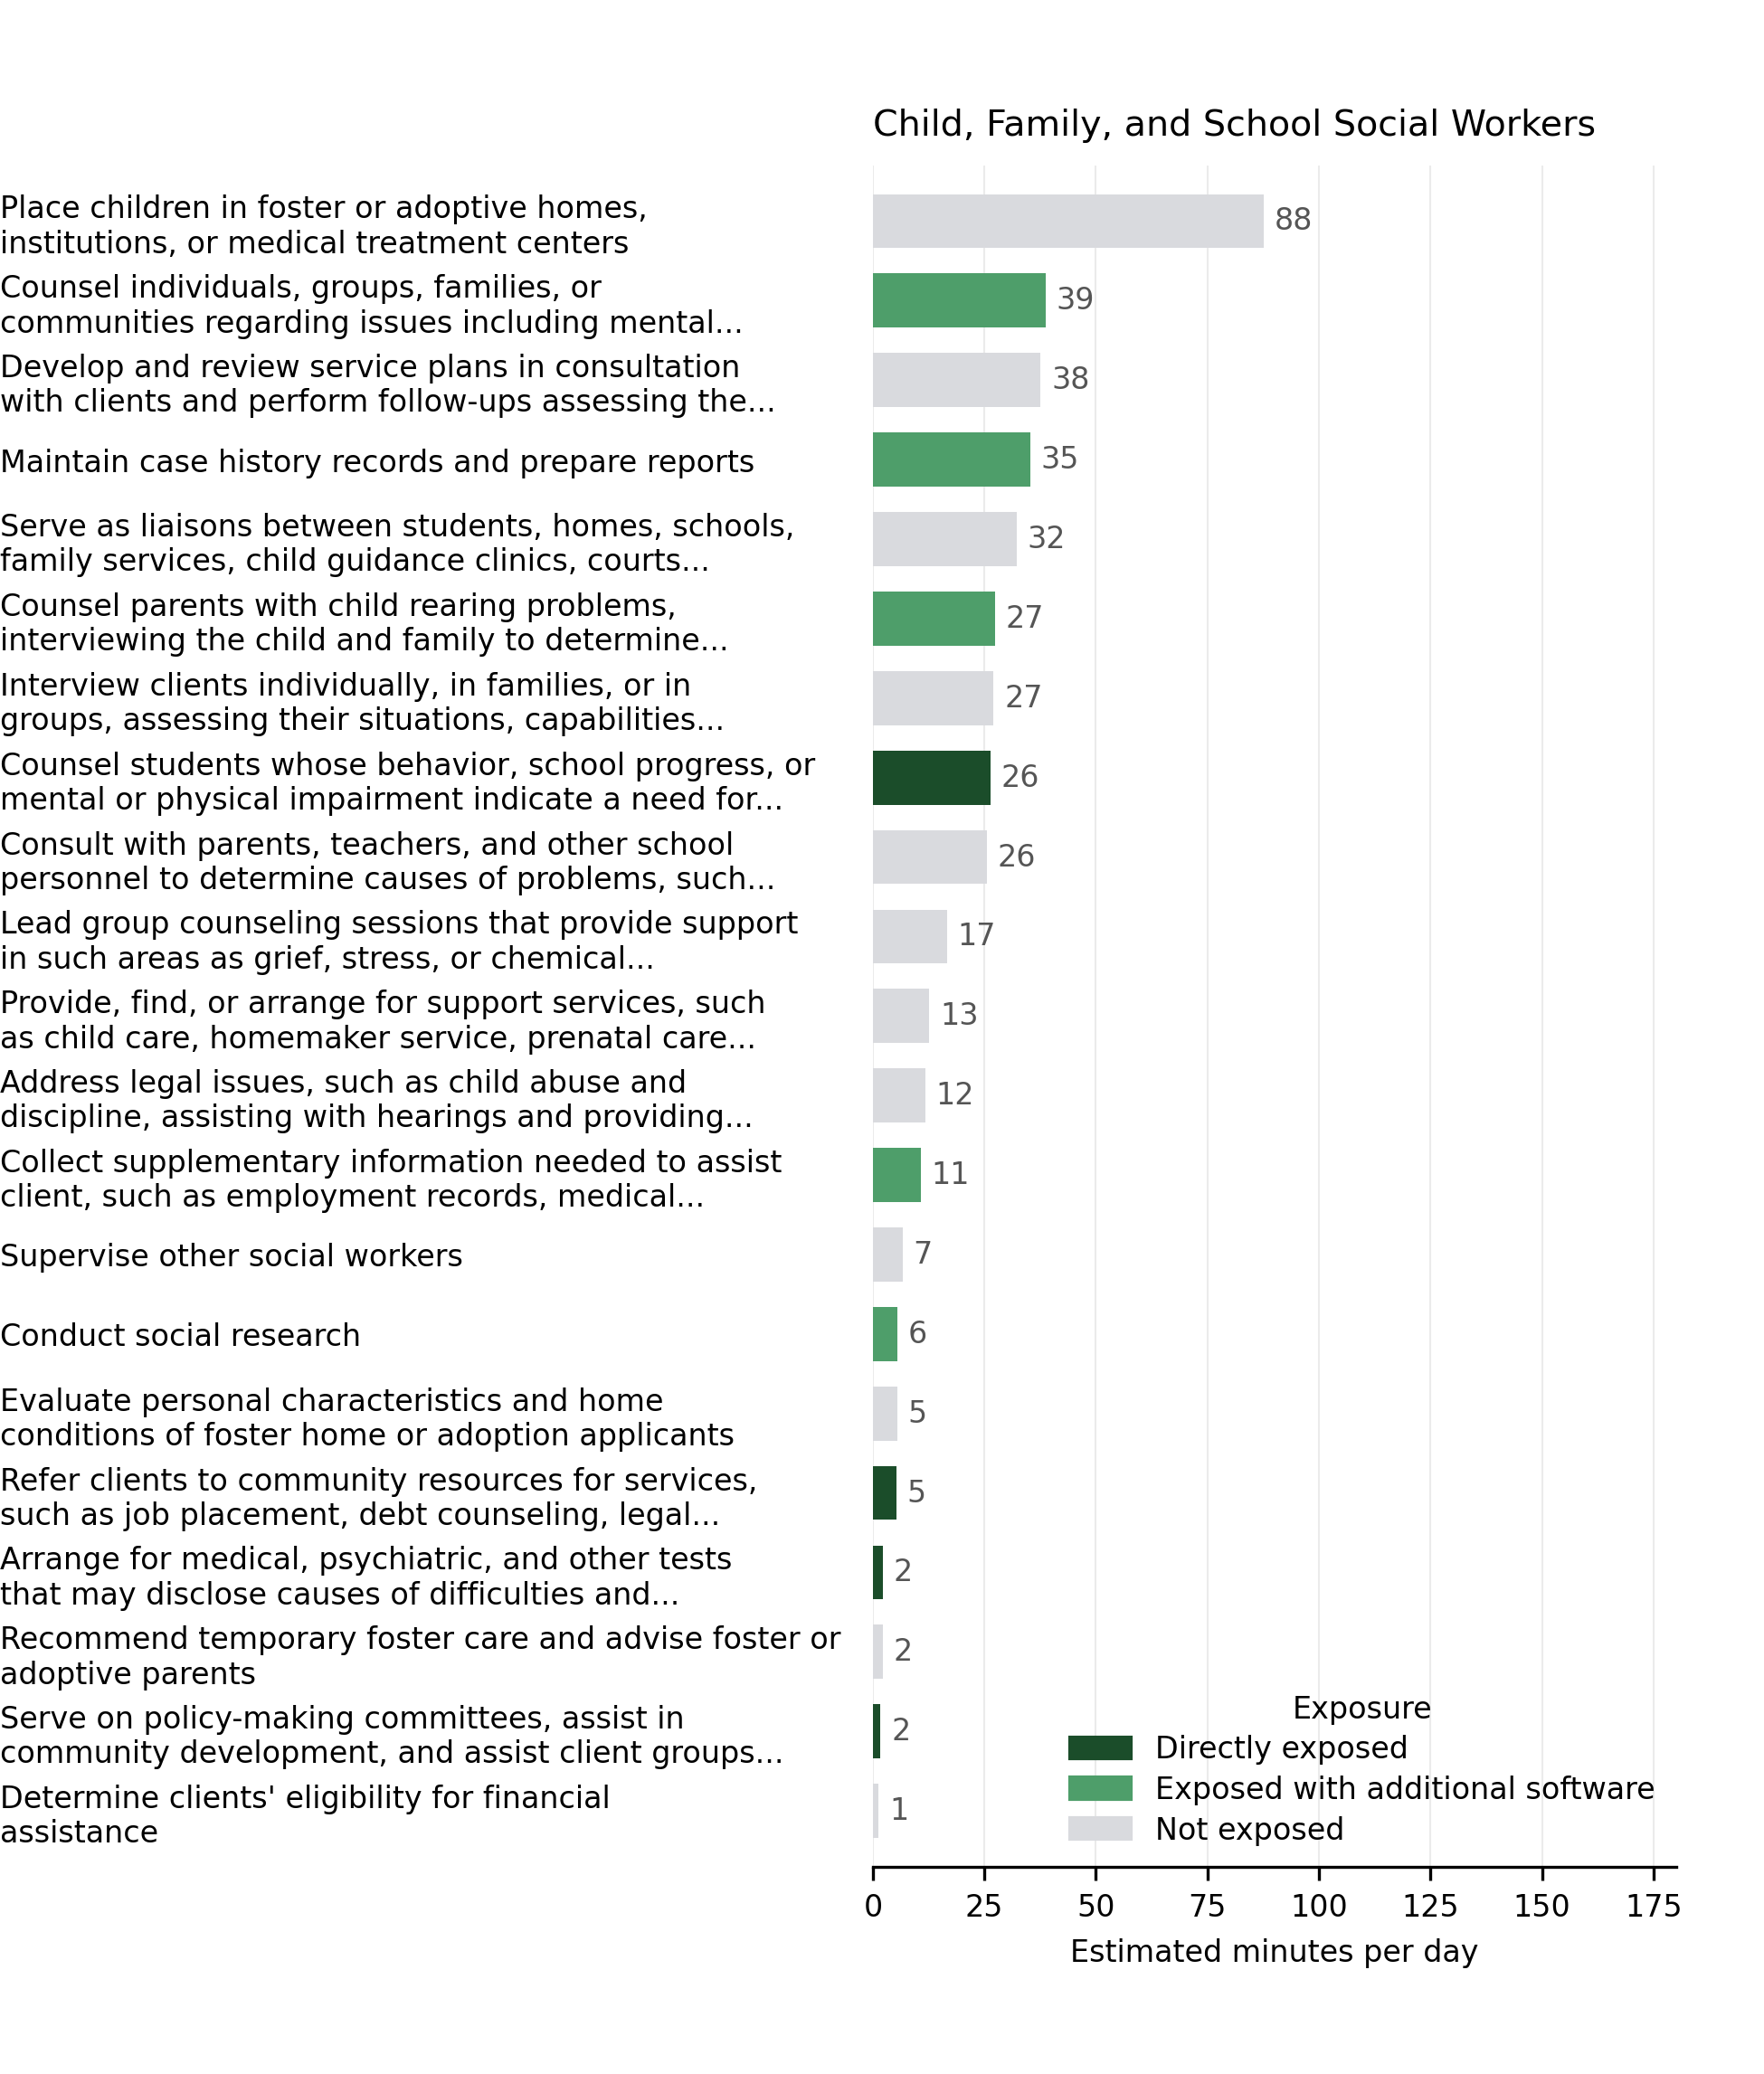
\includegraphics[width=0.8\textwidth]{figures/fig2_social_workers.png}
\caption*{Figure 2: Theoretical task-based exposure to AI for Child, Family, and School Social Workers. Ratings are human ratings from Eloundou et al. (2024); hours from Hatgis-Kessell et al. (2026).}
\end{figure}

Social and Community Service Managers show a different pattern from the two frontline occupations (Figure 3). Managers spend about a quarter of their workday (1 hour 41 minutes) directly exposed tasks. These tasks include establishing administrative procedures (49 minutes) and participating in determining organizational policy (21 minutes). An additional 3 hours 52 minutes of the managers 7-hour workday is considered partially exposed, of which one task, "Implement and evaluate staff, volunteer, or community training programs" accounts for 2 hours 51 minutes of this time. Only 1 hour 27 minutes of the managers' workday is considered not exposed.

\begin{figure}[!htbp]
\centering
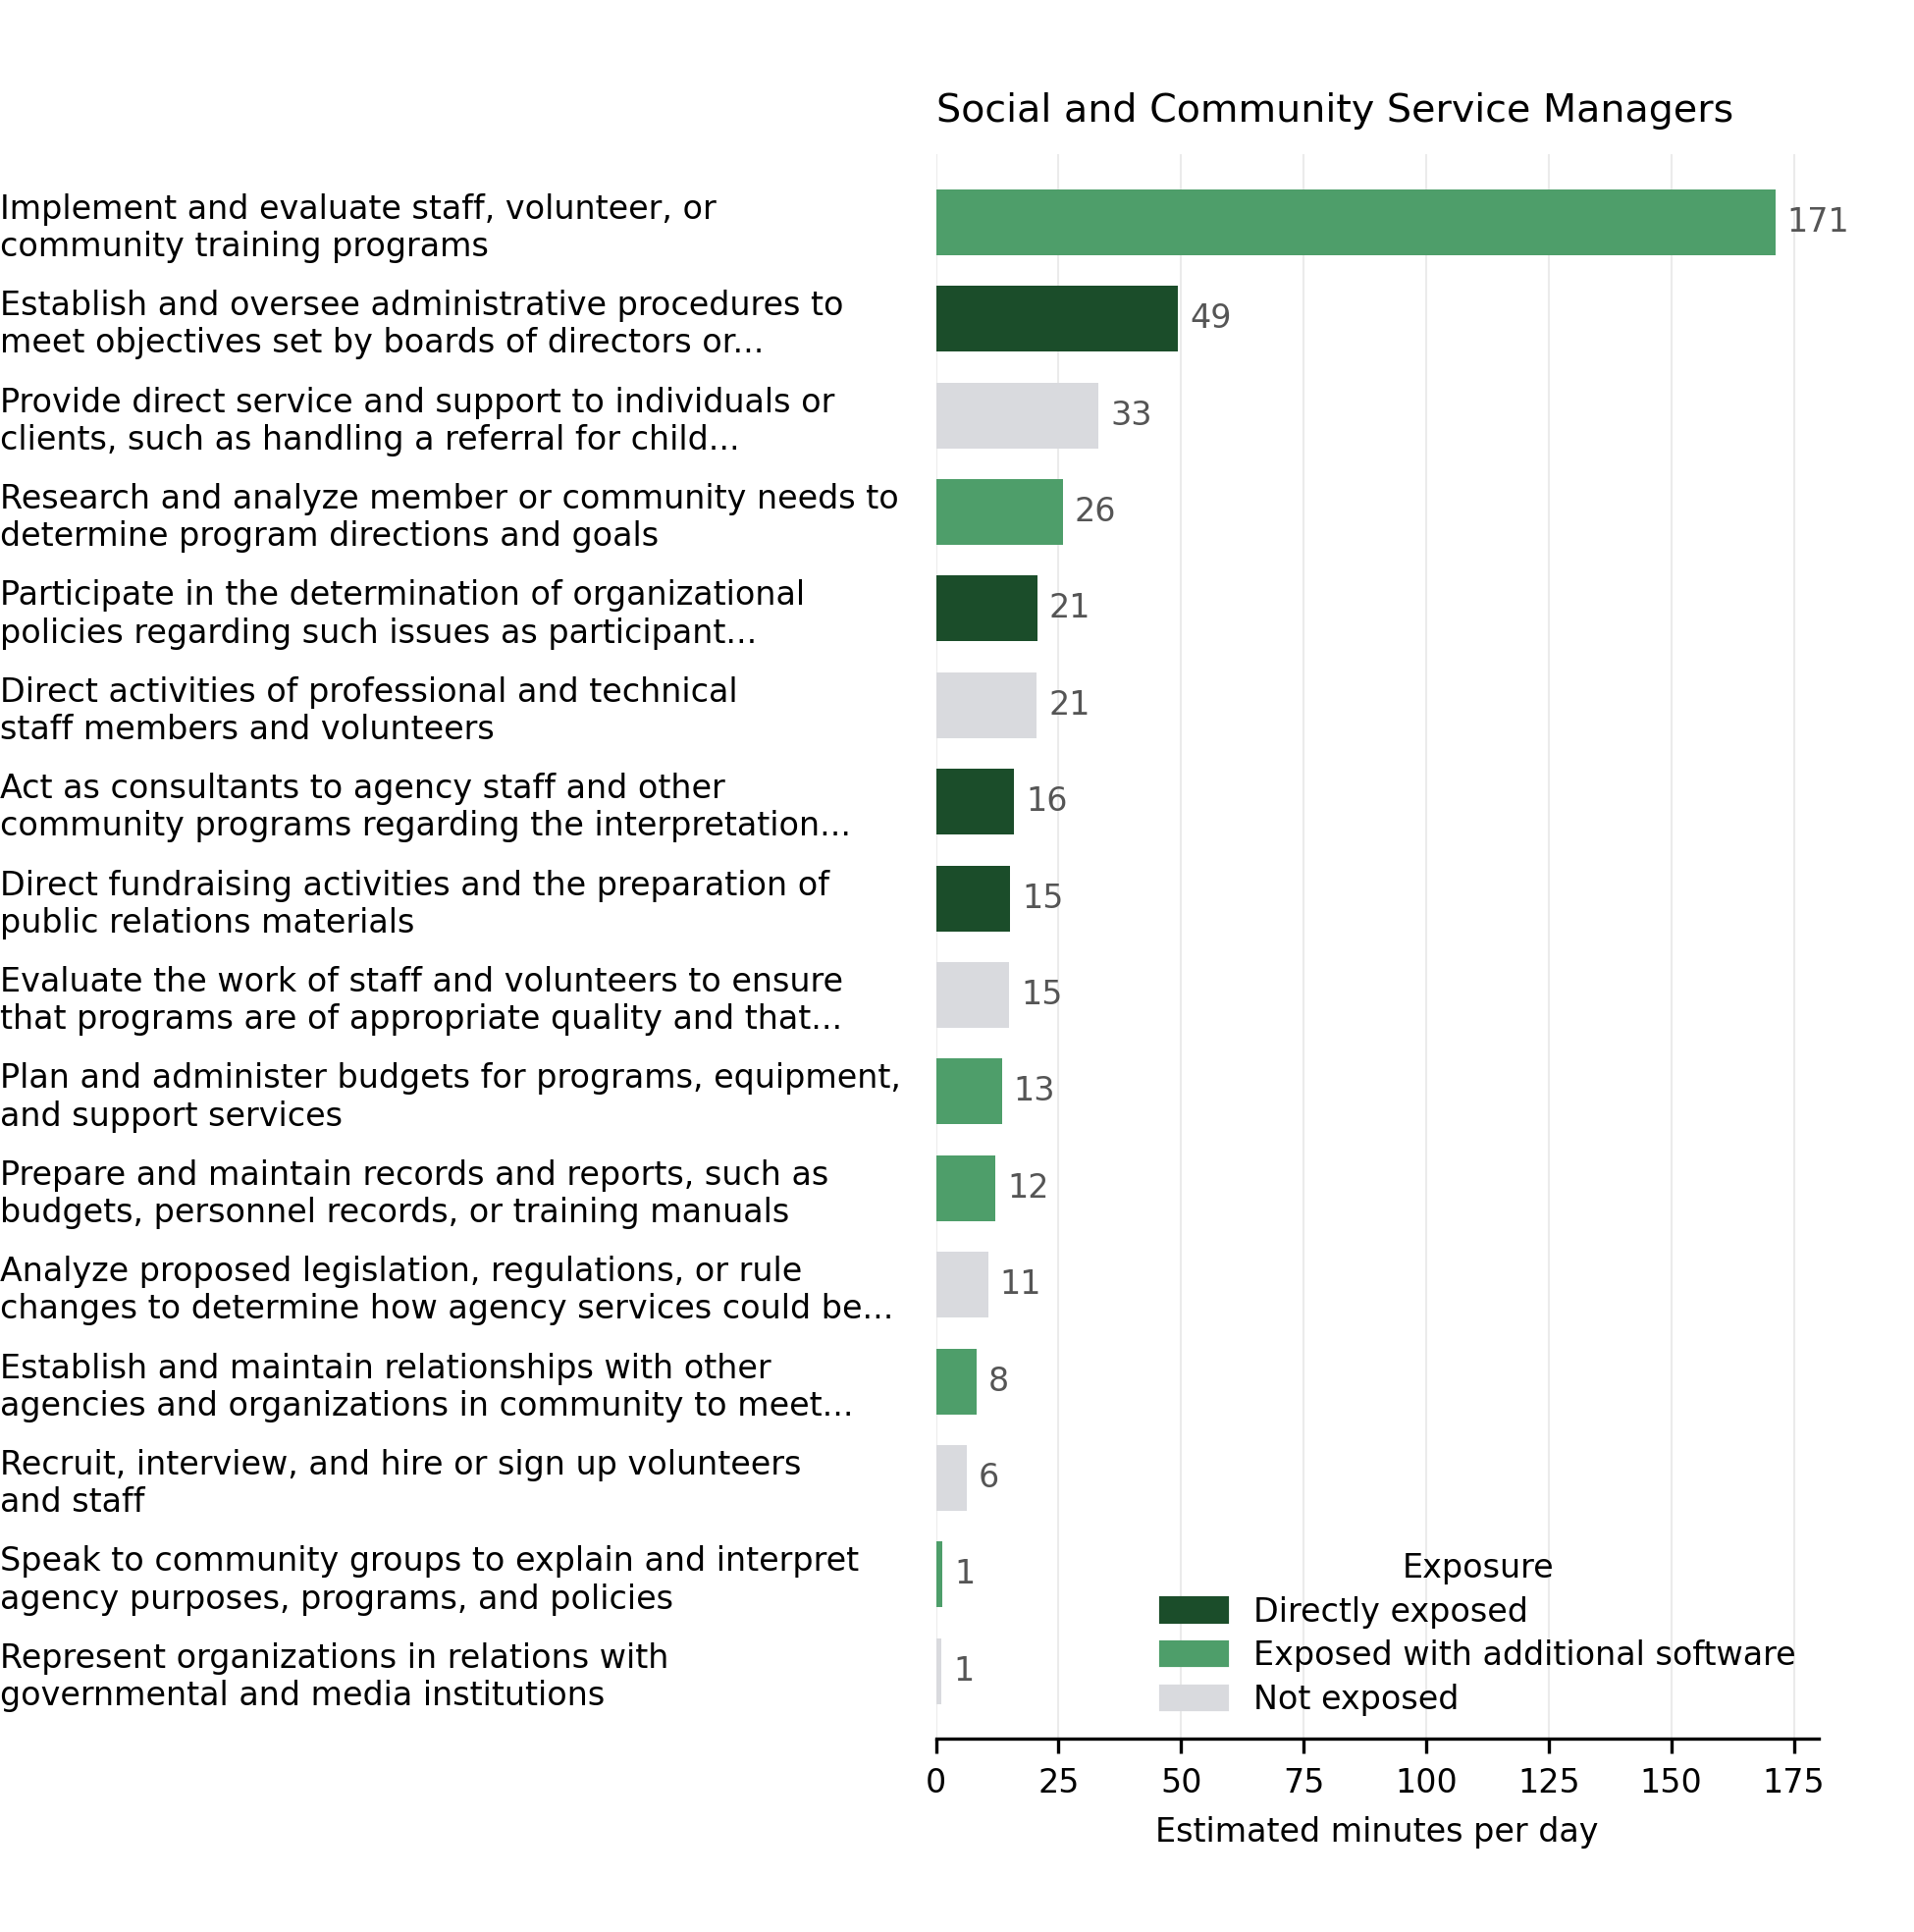
\includegraphics[width=0.8\textwidth]{figures/fig3_managers.png}
\caption*{Figure 3: Theoretical task-based exposure to AI for Social and Community Service Managers. Ratings are human ratings from Eloundou et al. (2024); hours from Hatgis-Kessell et al. (2026).}
\end{figure}

Job exposure to AI for each of the three occupations studied is summarized in Table 3. Managers have the most directly exposed time at 1 hour 41 minutes per day, while the two frontline workers show 24 and 36 minutes per day of directly exposed work. For all three occupations, time exposed only with additional software exceeds directly exposed time.

\begin{table}[!htbp]
\tablesize
\caption*{\textbf{Table 3.} Daily working time by exposure category.}
\begin{tabularx}{\textwidth}{@{}>{\raggedright\arraybackslash}X >{\raggedright\arraybackslash}p{2.5cm} >{\raggedright\arraybackslash}p{3.6cm} >{\raggedright\arraybackslash}p{2.3cm}@{}}
\toprule
& Time directly exposed (E1) & Time exposed with additional software (E2) & Time not exposed (E0) \\
\midrule
Social and Human Service Assistants & 0:24 (6\%) & 2:51 (41\%) & 3:45 (54\%) \\
Child, Family, and School Social Workers & 0:36 (8\%) & 1:58 (28\%) & 4:27 (64\%) \\
Social and Community Service Managers & 1:41 (24\%) & 3:52 (55\%) & 1:27 (21\%) \\
\bottomrule
\end{tabularx}
\tablenote{\emph{Note:} Time per 7-hour day in hours and minutes, with share of the day in parentheses. Human ratings from Eloundou et al. (2024).}
\end{table}

\subsection{Task counts versus time}

Weighting tasks by time changes how much of each occupation appears directly exposed to AI (Figure 4).

\begin{figure}[!htbp]
\centering
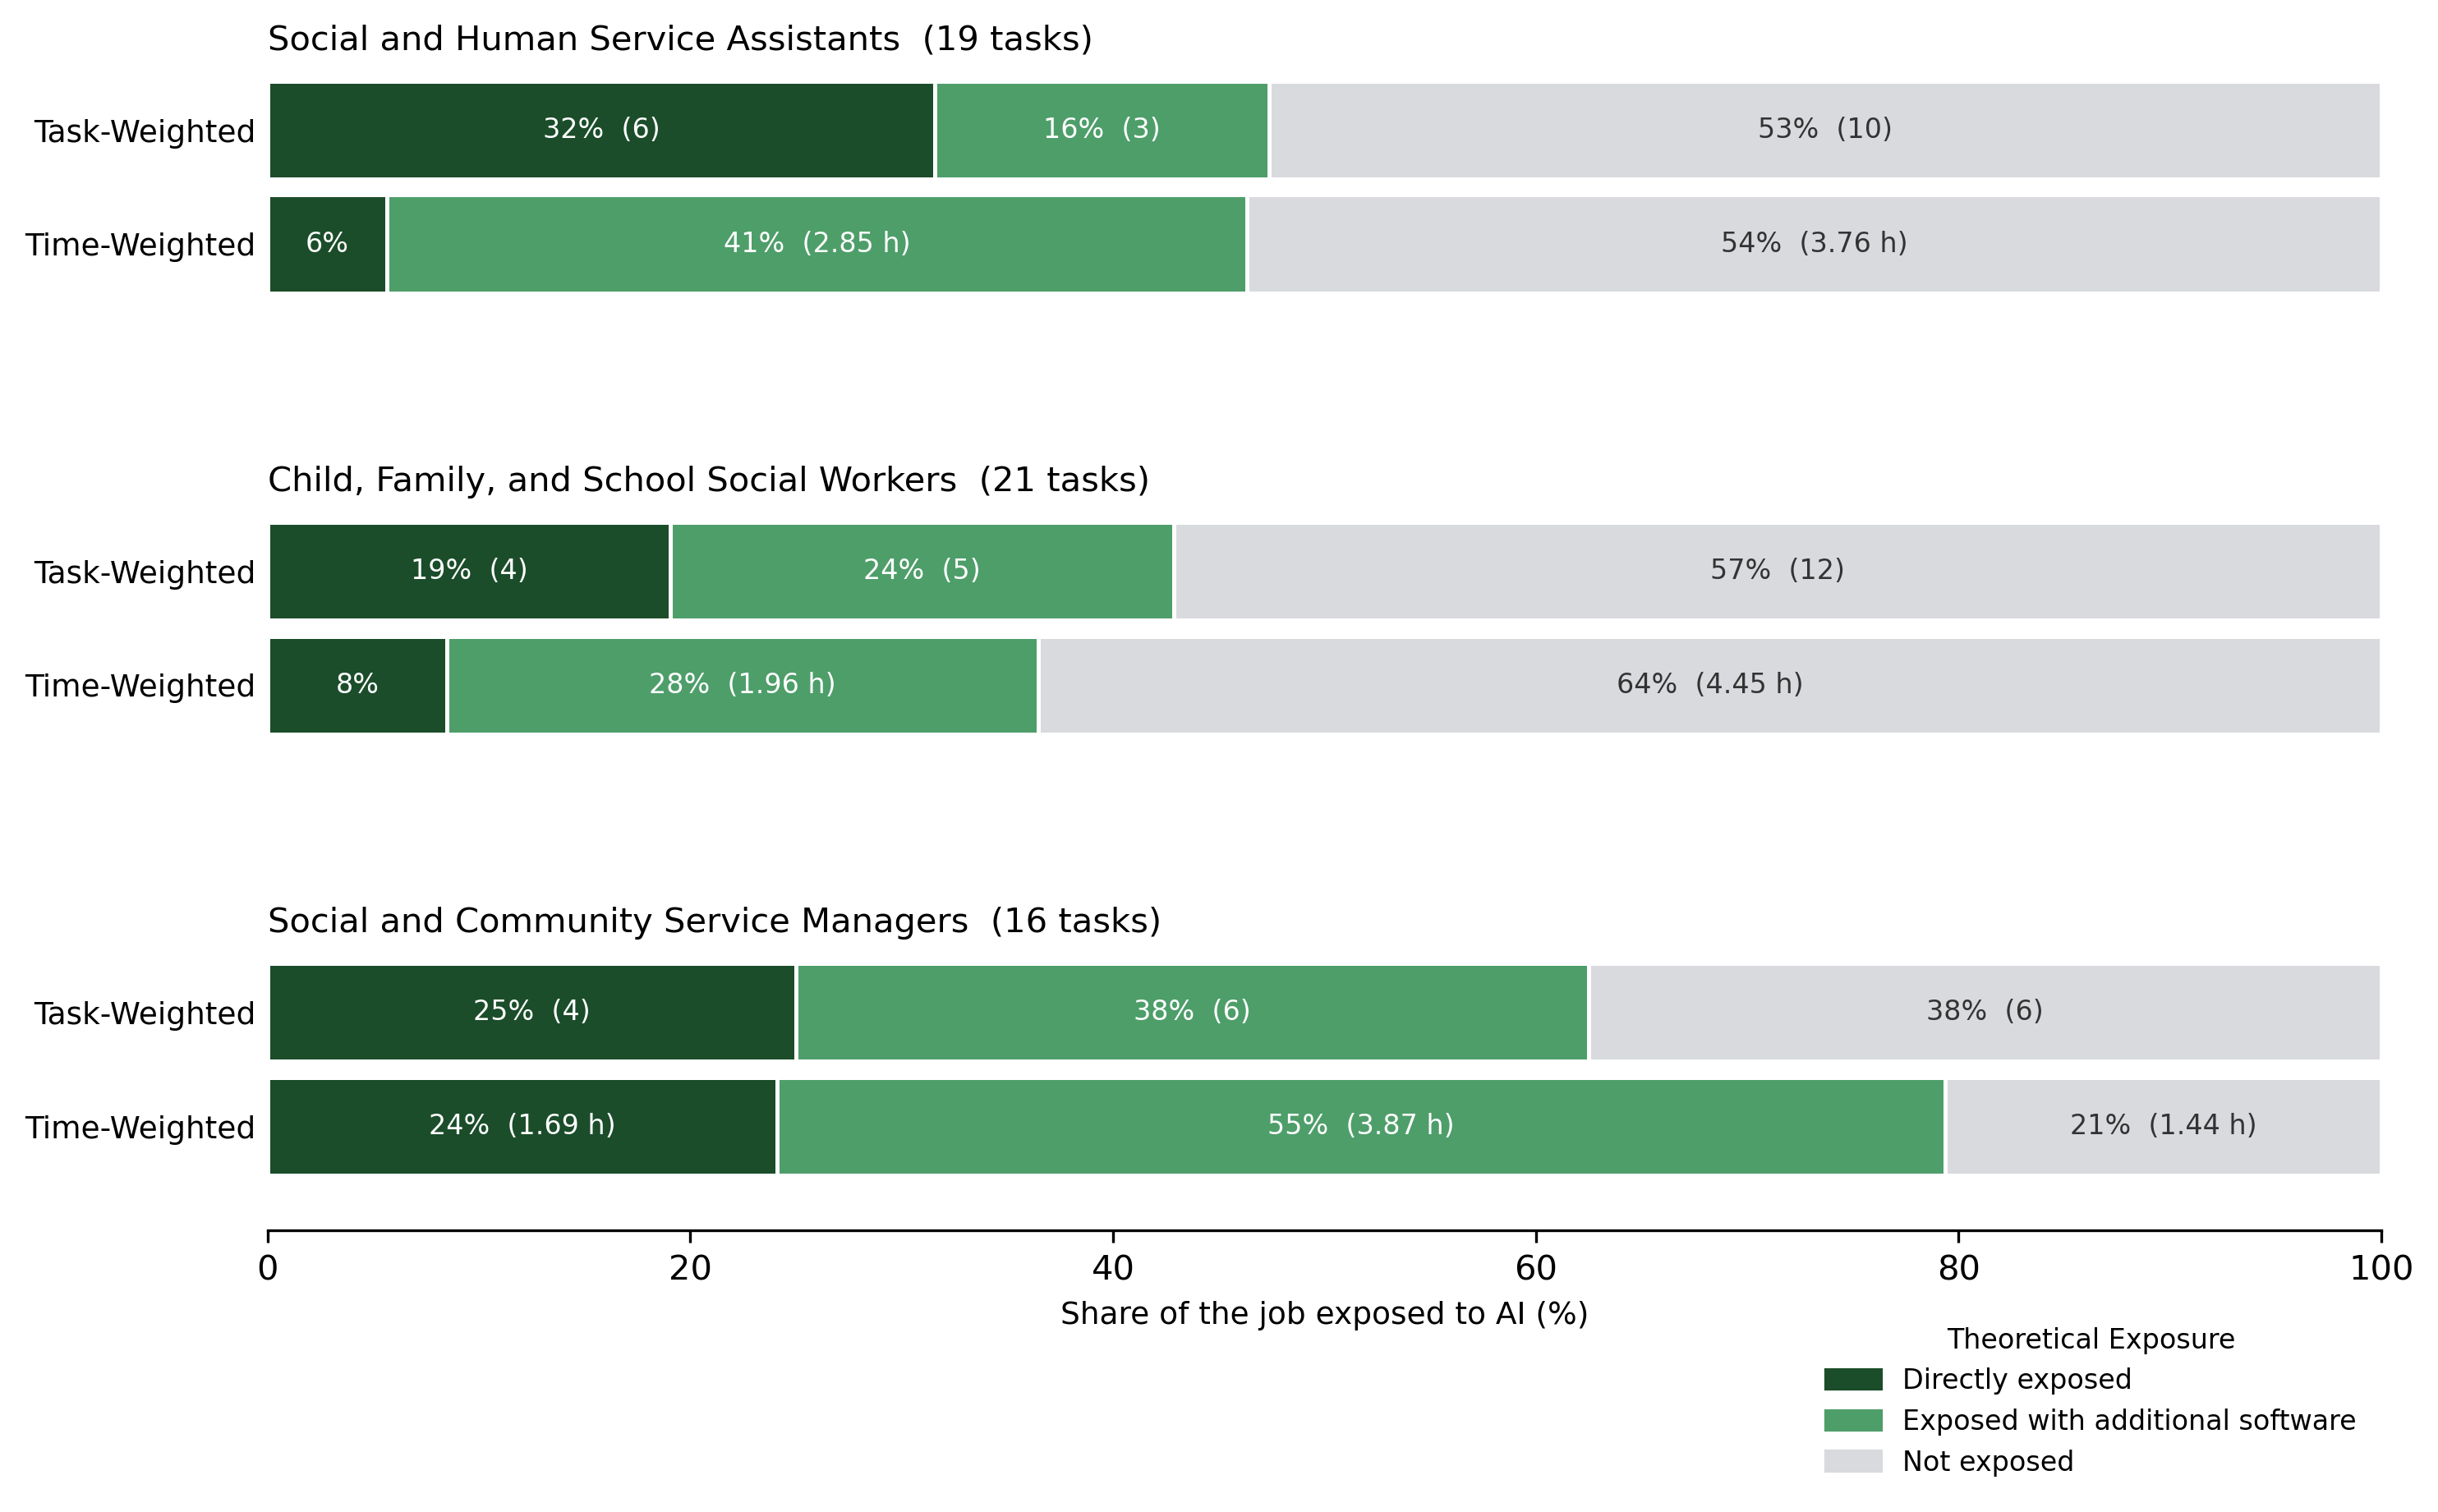
\includegraphics[width=1.0\textwidth]{figures/fig4_tasks_vs_time.png}
\end{figure}

For Social and Human Service Assistants, a third of tasks are directly exposed, but this translates to only 6 percent of the worker's day (Table 4). The total exposure (direct and partial exposure) is almost the same under both measures: 47 percent of tasks and 46 percent of time. What changes is its composition- a much greater share of the worker's day would require dedicated software in order to completely automate when considering the amount of time to complete tasks. The reason is that the directly exposed tasks are quick to do. The six of them average about 4 minutes a day each, while the three partially exposed (software-dependent) tasks average nearly an hour.

Child, Family, and School Social Workers show the same pattern on a smaller scale. Directly exposed work falls from 19 percent of tasks to 8 percent of time, while partially exposed work rises slightly, from 24 to 28 percent. The total exposure of Child, Family, and School Social workers falls from 43 to 36 percent when time-weighting is incorporated.

Social and Community Service Managers show a different pattern. Their directly exposed share is nearly the same under both exposure metrics. Their partially exposed share rises from 38 to 55 percent, because one task, "Implement and evaluate staff, volunteer, or community training programs," takes up 41 percent of the day. The total exposure of managers is therefore higher when time-weighting is considered, rising from 63 percent of tasks to 79 percent of time.

\subsection{Observed use}

Observed AI use, measured from Claude conversations in the workplace, reaches very few of the tasks in these occupations. Of the 56 tasks examined, four show work-related use above the reporting threshold, and together they account for a small share of the working day (Table 5).

\begin{table}[!htbp]
\tablesize
\caption*{\textbf{Table 5.} Tasks with observed AI use.}
\begin{tabularx}{\textwidth}{@{}>{\raggedright\arraybackslash}p{3.4cm} >{\raggedright\arraybackslash}X >{\raggedleft\arraybackslash}p{1.5cm} >{\raggedright\arraybackslash}p{2.5cm}@{}}
\toprule
Occupation & Task & Minutes per day & Exposure category \\
\midrule
Social and Human Service Assistants & None & 0 & n/a \\
Child, Family, and School Social Workers & Conduct social research & 6 & Partially exposed \\
Social and Community Service Managers & Research and analyze member or community needs to determine program directions and goals & 26 & Partially exposed \\
& Evaluate the work of staff and volunteers to ensure that programs are of appropriate quality and that resources are used effectively & 15 & Not exposed \\
& Prepare and maintain records and reports, such as budgets, personnel records, or training manuals & 12 & Partially exposed \\
\bottomrule
\end{tabularx}
\tablenote{\emph{Note:} Observed AI use from Massenkoff and McCrory (2026).}
\end{table}

None of the 19 tasks performed by Social and Human Service Assistants show observed use. For Child, Family, and School Social Workers, only 1 task does, and it occupies 6 minutes of the workday. For Social and Community Service Managers, three tasks of 16 show use. They occupy 53 minutes (about 13 percent of the mangers' workday).

The tasks with recorded use are not the ones rated as directly exposed. Three of the four are rated as partially exposed and one as not exposed. None of the 14 directly exposed tasks across the three occupations show recorded use.

\subsection{Worker hours}

Multiplied across each occupation's workforce, directly exposed time is modest for frontline staff and largest for managers (Table 6).

\begin{table}[!htbp]
\tablesize
\caption*{\textbf{Table 6.} Daily worker hours by exposure category.}
\begin{tabularx}{\textwidth}{@{}>{\raggedright\arraybackslash}X r >{\raggedleft\arraybackslash}p{2.2cm} >{\raggedleft\arraybackslash}p{2.3cm} >{\raggedleft\arraybackslash}p{2.1cm}@{}}
\toprule
Occupation & Total hours & Directly exposed hours & Partially exposed hours & Not exposed hours \\
\midrule
Social and Human Service Assistants & 253,750 & 14,273 (6\%) & 103,338 (41\%) & 136,139 (54\%) \\
Child, Family, and School Social Workers & 97,580 & 8,269 (8\%) & 27,308 (28\%) & 62,002 (64\%) \\
Social and Community Service Managers & 95,760 & 23,074 (24\%) & 52,924 (55\%) & 19,762 (21\%) \\
\bottomrule
\end{tabularx}
\end{table}

Social and Human Service Assistants work about a combined 253,750 hours a day, of which about 14,300 are spent on directly exposed tasks. For Child, Family, and School Social Workers the figure is about 8,300 of 97,600 hours across the workforce. Social and Community Service Managers account for the most directly exposed time, about 23,100 hours a day, although there are more than twice as many assistants (36,250 assistants) than managers in this sector (13,680 managers).

Because a directly exposed task is one that AI could complete in half the time or less, the minimum saving is half of these figures: about 7,100 hours a day for assistants, 4,100 for social workers, and 11,500 for managers.

In every occupation, the share of partially exposed time is much greater. For assistants it is about 103,300 hours a day, seven times their directly exposed time. I do not estimate a saving for partially exposed time, since it depends on software that has not been built.

\subsection{Sensitivity to rating source}

All results shown in this analysis were using human estimates of time to complete tasks. Here, the analysis is repeated using time to complete estimates judged by GPT-4 in order to test the sensitivity of the results. This sensitivity analysis leaves the frontline findings intact but changes the result for managers (Table 7).

\begin{table}[!htbp]
\tablesize
\caption*{\textbf{Table 7.} Daily hours by exposure category under human and GPT-4 ratings.}
\begin{tabularx}{\textwidth}{@{}>{\raggedright\arraybackslash}X >{\raggedright\arraybackslash}p{3.1cm} >{\raggedright\arraybackslash}p{3.2cm} >{\raggedright\arraybackslash}p{2.9cm}@{}}
\toprule
Occupation & Directly exposed (human / GPT-4) & Partially exposed (human / GPT-4) & Not exposed (human / GPT-4) \\
\midrule
Social and Human Service Assistants & 0:24 / 0:43 & 2:51 / 3:56 & 3:45 / 2:21 \\
Child, Family, and School Social Workers & 0:36 / 0:35 & 1:58 / 1:31 & 4:27 / 4:54 \\
Social and Community Service Managers & 1:41 / 0:12 & 3:52 / 5:45 & 1:27 / 1:03 \\
\bottomrule
\end{tabularx}
\tablenote{\emph{Note:} Both sets of ratings are from Eloundou et al. (2024).}
\end{table}

The two sets of ratings agree on 29 of the 56 tasks (52 percent). They disagree most about which tasks are directly exposed. Human judges rated 14 tasks as directly exposed- the GPT-4 judge was more cautious: it agreed on only 3 of them, rating 9 of the others as partially exposed and 2 as not exposed.

For the two frontline occupations, the main finding holds under either rating. Directly exposed time is under an hour a day: 24 minutes according to a human judge and 43 minutes with a GPT-4 judge for Social and Human Service Assistants, and 36 and 35 minutes under both judges for Child, Family, and School Social Workers. In both occupations, partially exposed time is several times larger than directly exposed time whether a human rating or GPT-4 rating is used.

For Social and Community Service Managers, the result depends on the rating. Directly exposed time is 1 hour 41 minutes when judged by humans and 12 minutes when judged by GPT-4, with the difference moving almost entirely into the partially exposed category. The two sets of judges agree on the exposure category for only 5 of the 16 managerial tasks.

\section{Discussion}

This article asked how much of the working day in the three largest community service occupations is spent on tasks that current AI can realistically speed up. The analysis shows that directly exposed tasks make up a small part of that day. Social and Human Service Assistants and Child, Family, and School Social Workers each spend less than an hour a day on them. A larger share of the day falls on partially exposed tasks, which AI could speed up only with software built for the purpose. This pattern holds all three occupations, and under both human and GPT-4 ratings, where a larger portion of the workday is partially exposed rather than directly exposed.

The measured exposure of community service work to AI depends on how exposure is counted. When tasks are counted equally, 32 percent of the work of Social and Human Service Assistants is directly exposed to AI. When tasks are weighted by time, the figure is just 6 percent of their day. The tasks in this occupation that an LLM could accelerate without additional software, such as referring clients to other agencies or submitting reports to a supervisor, occupy little of the working day. This result is consistent with Hatgis-Kessell et al. (2026), who find across the economy that time weighting reduces the contribution of short, transactional tasks. Task-based measures therefore yield a more favorable estimate of what AI can immediately offer these occupations than time-based measures do.

Most of the exposed time in these occupations is partially exposed, and it is concentrated in a small number of long tasks. For Social and Human Service Assistants, a single task, developing and implementing care plans, accounts for almost two-thirds of partially exposed time. Under the definition used by Eloundou et al. (2024), such tasks could be accelerated only if additional software were built on an LLM. The larger share of potential time savings in these occupations is therefore not accessible through general-purpose AI tools. It is conditional on software that would need to be developed, funded, and maintained.

Observed use was recorded to only four tasks across all three occupations. None of the four tasks were rated as directly exposed. This should not be interpreted as evidence that this workforce does not use AI. The observed use metric from Massenkoff and McCrory (2026) covers only one platform (Claude), and 64 percent of surveyed social workers report that they are using AI in their work (Borah et al. 2026). It does indicate that observed use has not occurred on the tasks the tasks that were rated as the most theoretically exposed.

\setcounter{subsection}{1} % keeps the draft numbering (5.2)

\subsection{Implications for policy and practice.}

\emph{For nonprofit managers.} These results suggest that general-purpose AI tools, used without additional software, are likely to return a limited amount of frontline staff time. Under the human ratings, the minimum saving on directly exposed tasks is about 12 minutes a day for a Social and Human Service Assistant and about 18 minutes for a Child, Family, and School Social Worker. Savings of this size may be worthwhile, but they are unlikely to offset the staffing shortfalls described in Section 2. Managers who expect AI to relieve frontline workloads should distinguish between tasks that current tools can accelerate, which are brief, and the longer tasks, such as care planning and case recording, that would require software designed to augment the LLM.

\emph{For funders.} Most of the working time that AI could affect in these occupations is partially exposed, and it is concentrated in a small number of tasks that are common across organizations. Few local community service organizations have the capacity to commission software or get specialized training for AI adoption (Smith Arrillaga, Grundhoefer, and Im 2025). Custom-built software with AI features are not common in this sector: just 5 percent of social workers describe using such software for case management (Borah et al. 2026). Building dedicated software for time-consuming tasks such as care planning may therefore return more staff time than support for individual licenses to general-purpose AI chat products.

\emph{For policymakers}. The single largest partially exposed tasks in the frontline occupations (care planning and case recording) likely can only be accelerated only with dedicated software built to extend the LLM. Agencies that require grantees to use specific data systems should look for ways to support AI features inside of those systems. Guidance on the use of client information in AI tools would address the barriers social workers cite most often, ethics and data privacy (Borah et al. 2026).

\subsection{Limitations}

The findings depend on three published measures, each with limitations. The exposure ratings date from early 2023 and are subjective: human and GPT-4 ratings agree on about half of the tasks examined, and the result for managers differs widely between them (Section 4.5). The time estimates are generated by a language model, not observed, and assign a large share of the day to single tasks. The measure of observed use covers one AI product and records a task only above a minimum volume, so it understates use to an unknown degree.

The scope of the analysis is also limited. Employment data are available only for the industry group as a whole, which includes for-profit employers and organizations outside the population of interest. The three occupations examined account for 27.6 percent of the industry's jobs, and the results should not be generalized to the sector. Estimates of total worker hours treat every job as full-time and exclude volunteers, who are common in food and shelter organizations.

\section{Conclusion}

This article examined how much of the working day in the three largest occupations in community food, housing, and relief services is spent on tasks that AI can perform. Tasks that an LLM could accelerate without additional software account for less than an hour of the frontline working day. A larger share falls on tasks that would require software built for the purpose, and observed AI use reaches few tasks in these occupations. For organizations facing staff shortages, general-purpose AI tools are therefore likely to offer modest relief. There is greater potential in offloading worker burden via custom software built to support the task.

The article contributes a time-weighted account of AI exposure dedicated to the local community service relief sector. The article shows that measures based on counts of tasks versus time-weighted results may lead to different conclusions. Future research could test these estimates through direct time-use studies dedicated to the occupations at hand and also through usage data from more than one AI product. Studies of AI in the nonprofit sector would also benefit from recording which tasks AI is used for and how much working time those tasks occupy.

\section*{Data and code availability}

This study uses publicly available data from the U.S. Bureau of Labor Statistics (2026). Data published by Eloundou et al. (2024), Hatgis-Kessell et al. (2026), and the Anthropic Economic Index (Anthropic 2026) were also used. No new data were collected. The code used to download the data and reproduce all figures is available at \url{https://github.com/shannongross/ai-workforce-exposure}.
   % not in the Word draft; edit this file directly
\section*{Disclosure statement}

The author conducted this research independently and is solely responsible for its content. AI was used in fine-tuning wording, but the work is original and not ai-generated. The author received no funding for this work and reports no competing interests.

\section*{References}
\begin{reflist}

\item Anthropic. 2026. "Anthropic Economic Index." Dataset. Hugging Face. Accessed September 27, 2026. \url{https://huggingface.co/datasets/Anthropic/EconomicIndex}.

\item Borah, Elisa, Jillian Meyerhoff, Akram Al-Turk, Katherine Gower, and Anna Mastryukova. 2026. \emph{Use of Artificial Intelligence in Social Work Practice: Findings and Recommendations from a National Survey}. Austin: Moritz Center for Societal Impact, School of Social Work, University of Texas at Austin. \url{https://moritzcenter.utexas.edu/wp-content/uploads/2026/06/Moritz-Center-AI-SW-Survey-Report.pdf}.

\item Eloundou, Tyna, Sam Manning, Pamela Mishkin, and Daniel Rock. 2024. "GPTs Are GPTs: Labor Market Impact Potential of LLMs." \emph{Science} 384 (6702): 1306--8. \url{https://doi.org/10.1126/science.adj0998}.

\item Grundhoefer, Seara, Elisha Smith Arrillaga, and Ellie Buteau. 2026. \emph{State of Nonprofits 2026: What Funders Need to Know}. Cambridge, MA: Center for Effective Philanthropy. \url{https://cep.org/wp-content/uploads/2026/05/CEP_State_of_Nonprofits_2026_FNL.pdf}.

\item Hatgis-Kessell, Stephane, Tomás Aguirre, Alexander Wan, and Rishi Bommasani. 2026. "Estimating Time Spent on Work Tasks." Preprint, arXiv, June 26. \url{https://arxiv.org/abs/2608.05172}.

\item Martin, Hannah. 2026. "Funding Challenges, Increasing Demand Drive Staff Burnout Concerns." \emph{Candid Insights} (blog), April 14. \url{https://candid.org/blogs/nonprofit-staff-burnout/}.

\item Massenkoff, Maxim, and Peter McCrory. 2026. "Labor Market Impacts of AI: A New Measure and Early Evidence." Anthropic, March 5. \url{https://www.anthropic.com/research/labor-market-impacts}.

\item National Center for Charitable Statistics. 2025. "National Taxonomy of Exempt Entities (NTEE) Codes." Urban Institute. Accessed September 30, 2026. \url{https://nccs.urban.org/nccs/datasets/ntee/}.

\item National Center for O*NET Development. 2026. "O*NET 31.0 Database." O*NET Resource Center. Accessed September 27, 2026. \url{https://www.onetcenter.org/database.html}.

\item Nonprofit Finance Fund. 2025. \emph{2025 National State of the Nonprofit Sector Survey Findings: Essential, Enduring, and Under Strain}. New York: Nonprofit Finance Fund. \url{https://nff.org/wp-content/uploads/NFF-2025-Survey-Report.pdf}.

\item NTEN and The Bridgespan Group. 2026. \emph{State of Nonprofit AI Adoption and Governance}. Portland, OR: NTEN. \url{https://content.nten.org/wp-content/uploads/2026/09/2026-State-of-Nonprofit-AI.pdf}.

\item Shi, Wanzhu, and Lauren Azevedo. 2026. "Determinants of AI Adoption in Nonprofit Organizations." \emph{Nonprofit and Voluntary Sector Quarterly}. Published ahead of print, March 30. \url{https://doi.org/10.1177/08997640261429018}.

\item Smith Arrillaga, Elisha, Seara Grundhoefer, and Christina Im. 2025. \emph{AI With Purpose: How Foundations and Nonprofits Are Thinking About and Using Artificial Intelligence}. Cambridge, MA: Center for Effective Philanthropy. \url{https://cep.org/wp-content/uploads/2025/09/CEP_AI_Layout_FINAL.pdf}.

\item TechSoup and Tapp Network. 2025. \emph{The State of AI in Nonprofits: 2025}. San Francisco: TechSoup. \url{https://pages.techsoup.org/hubfs/Downloads/The\%20State\%20of\%20AI\%20in\%20Nonprofits\%202025.pdf}.

\item U.S. Bureau of Labor Statistics. 2026. "Occupational Employment and Wage Statistics, May 2025: National Industry-Specific Estimates." \url{https://www.bls.gov/oes/}.

\end{reflist}


% The draft ends with two empty headings, "Figure captions" and "Appendix".
% They are left out of the PDF until they have content.
\end{document}
